\documentclass[tikz,border=5pt]{standalone}
\usepackage[utf8]{inputenc}
\usepackage[T1]{fontenc}
\usepackage{lmodern,amsmath,amssymb}
\usepackage[american]{circuitikz}
\usepackage{pgfplots}
\pgfplotsset{compat=1.18}
\usetikzlibrary{circuits.logic.US,positioning,calc,arrows.meta,patterns,shapes.geometric}
\definecolor{Primary}{HTML}{1F77B4}
\begin{document}
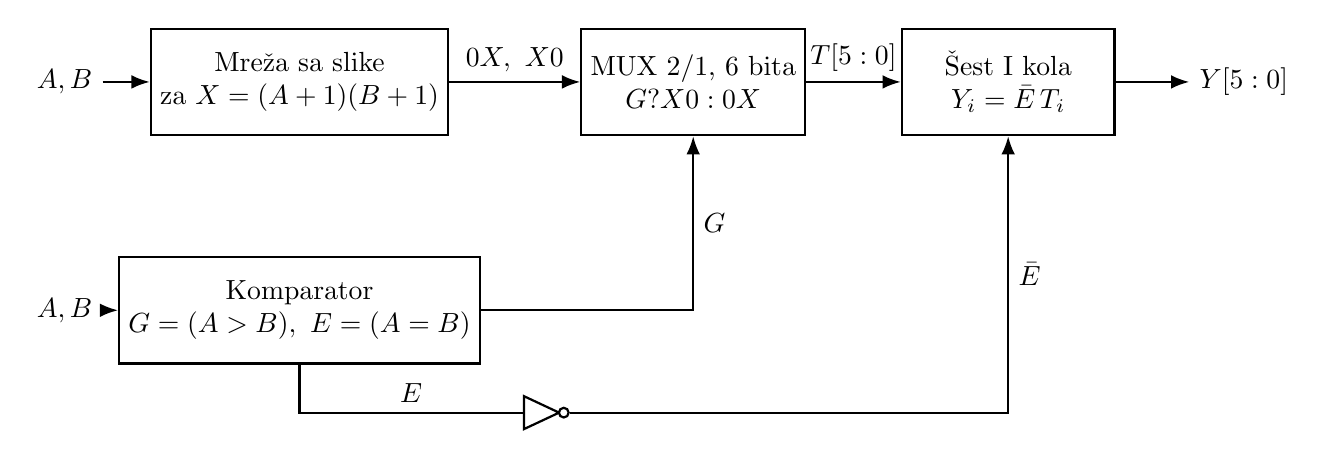
\begin{tikzpicture}[circuit logic US,thick,>=Latex,b/.style={draw,minimum width=2.7cm,minimum height=1.35cm,align=center}]
\node[b](x)at(0,1.5){Mreža sa slike\\za $X=(A+1)(B+1)$};
\node[b](c)at(0,-1.4){Komparator\\$G=(A>B),\ E=(A=B)$};
\node[b](mux)at(5,1.5){MUX 2/1, 6 bita\\$G?X0:0X$};\node[b](mask)at(9,1.5){Šest I kola\\$Y_i=\bar E\,T_i$};
\draw[->](-2.5,1.5)node[left]{$A,B$}--(x);\draw[->](-2.5,-1.4)node[left]{$A,B$}--(c);
\draw[->](x)--(mux)node[midway,above]{$0X,\ X0$};\draw[->](mux)--(mask)node[midway,above]{$T[5:0]$};\draw[->](mask)--++(2.3,0)node[right]{$Y[5:0]$};
\draw[->](c.east)--(5,-1.4)--(mux.south)node[midway,right]{$G$};\node[not gate US,draw] (ne) at (3,-2.7){};
\draw(c.south)--(0,-2.7)--(ne.input)node[midway,above]{$E$};
\draw[->](ne.output)--(9,-2.7)--(mask.south)node[midway,right]{$\bar E$};
\end{tikzpicture}
\end{document}
